%%%%%%%%%%%%%%%%%%%
%% additive-codes.tex
%%%%%%%%%%%%%%%%%%

The theory of quantum error correcting code
is an important cornerstone for fault-tolerant quantum computers~\cite{Shor1996Fault-tolerant,Preskill1998Fault-tolerant}.
One encodes states one wish to compute about into logical many-qubit states
in such a way that errors that are likely to happen will be correctable.
Thus, at the logical level an effective error rate is much smaller than the physical error rate.
Computation can be carried on this logical level,
and the overhead of error correction can be controlled, not to overwhelm the promised computation.
After the discovery of the very first quantum error correcting code by Shor~\cite{Shor1995nine},
people have quickly realized analogy between classical error correcting codes and a class of quantum error correcting codes%
~\cite{CalderbankRainsShorEtAl1997Quantum,Gottesman1996Saturating},
which are now known as additive or stabilizer codes.
Arguably, it is the most studied class of codes, and is the main object of the present thesis.
The connection between the classical codes and quantum additive codes is provided
by the parameterization of basis operators (Pauli matrices) by binary numbers.
In this chapter we review and exploit this correspondence.

The chapter is organized as follows.
Section~\ref{sec:pauli-group-symplectic-vector-space} provides a convenient and important viewpoint
under which the multiplicative group of all Pauli matrices are described by a vector space over the binary field.
Section~\ref{sec:additive-stabilizer-codes} builds on this viewpoint and explains how to choose a subspace
of a many qubit Hilbert space, which we hope to have a capability to correct errors.
Section~\ref{sec:cleaning-lemma} is devoted to derive an equation, called a cleaning lemma,
that relates the numbers of logical operators 
that can be supported on complementary regions and the total number of logical qubits.
It is remarked that the cleaning lemma implies 
that any error occurring within a region, where no nontrivial logical operator can be supported,
can actually be corrected by a physical operation.

The last section~\ref{sec:subsystem-tradeoff}
presents an application of the cleaning lemma 
which gives a constraint on the geometric shape of logical operators of local codes on lattices.
Most importantly, it is proved that in two-dimensional lattice codes with geometrically local generators with large code distance,
all logical operators have representatives supported on narrow strips.
It had been known by Bravyi and Terhal~\cite{BravyiTerhal2009no-go} 
that there exists a nontrivial logical operator supported on a strip.
Our conclusion extends this result by finding the geometric shape of \emph{all} logical operators.
If the minimal weight logical operator has weight proportional to the linear dimension of a two-dimensional system,
then all logical operator can be found on narrow strips~\cite{HaahPreskill2012tradeoff}.


Note that there are many interesting quantum codes that are not necessarily additive~\cite{
RainsHardinShorSloane1997Nonadditive,
Kitaev2003Fault-tolerant,
LevinWen2005String-net},
but they are out of the scope of this thesis.

\section{Pauli group as a symplectic vector space}
\label{sec:pauli-group-symplectic-vector-space}

The Pauli matrices
\[
 \sigma^x = \begin{pmatrix} 0 & 1 \\ 1 & 0 \end{pmatrix}, \quad
 \sigma^y = \begin{pmatrix} 0 & -i \\ i & 0 \end{pmatrix}, \quad
 \sigma^z = \begin{pmatrix} 1 & 0 \\ 0 & -1 \end{pmatrix}
\]
satisfy
\[
 \sigma_a \sigma_b = i \varepsilon_{abc} \sigma_c, \quad
 \{ \sigma_a , \sigma_b \} = 2 \delta_{ab}.
\]
Thus, the Pauli matrices together with scalars $\pm 1, \pm i$
form a group under multiplication.
Given a system of qubits,
the set of all possible tensor products of the Pauli matrices form a group,
where the group operation is the multiplication of operators.
If the system is infinite, physically meaningful operators
are those of finite support, i.e.,
acting on all but finitely many qubits by the identity.
We shall only consider this Pauli group of finite support,
and call it simply the {\bf Pauli group}.
An element of the Pauli group is called a {\bf Pauli operator}.
When finitely many qubits are considered,
a Pauli operator is of course an \emph{arbitrary} tensor product of Pauli matrices.


Since any two elements of the Pauli group either commute or anti-commute,
ignoring the phase factor altogether, one obtains an {\em abelian} group.
Moreover, since any element $O$ of the Pauli group satisfies $O^2 = \pm I$,
an action of $\mathbb{Z}/2\mathbb{Z}$ on Pauli group modulo phase factors
$P / \{\pm 1, \pm i\}$ is well-defined,
by the rule $ n \cdot O = O^n$ where $n \in \mathbb{Z}/2\mathbb{Z}$.
For $\FF_2 = \mathbb{Z}/2\mathbb{Z}$ being a field,
$P / \{\pm 1, \pm i\}$ becomes a vector space over $\FF_2$.
The group of single-qubit Pauli operators up to phase factors
is identified with the two-dimensional $\FF_2$-vector space.
If $\Lambda$ is the index set of all qubits in the system,
the whole Pauli group up to phase factors is the direct sum $\bigoplus_{i \in \Lambda} V_i$,
which we call {\bf Pauli space},
where $V_i$ is the vector space of the Pauli operators for the qubit at $i$.
Explicitly, $I = (00), \sigma^x = (10), \sigma^z = (01), \sigma^y = (11)$.
A multi-qubit Pauli operator
is written as a finite product of the single-qubit Pauli operators,
and hence is written as a binary string in which all but finitely many entries are zero.
A pair of entries of the binary string describes a single-qubit component in the tensor product expression.
The multiplication of two Pauli operators corresponds to entry-wise addition of the two binary strings modulo 2.


The commutation relation may seem at first lost,
but one can recover it by introducing a symplectic form~\cite{CalderbankRainsShorEtAl1997Quantum}.
Let
\[
 \lambda_1 = \begin{pmatrix} 0 & 1 \\ -1 & 0 \end{pmatrix}
\]
be a symplectic form on the vector space $(\FF_2)^2$ of single-qubit Pauli operators.%
%
\footnote{The minus sign is not necessary for qubits, but is for qudits of prime dimensions.}
%
One can easily check that the commutation relation of two Pauli matrices $O_1, O_2$
is precisely the value of this symplectic form
evaluated on the pair of vectors representing $O_1$ and $O_2$.
Two multi-qubit Pauli operator (anti-)commutes, if and only if
there are (odd) even number of pairs of the anticommuting single-qubit Pauli operators
in their tensor product expression.
Therefore, the two Pauli operator \mbox{(anti-)}commutes
precisely when the value of the direct sum of symplectic form $\bigoplus_{q \in \Lambda} \lambda_1$ is \mbox{(non-)}zero. 
$\Lambda$ could be infinite but the form is well-defined since any vector representing a Pauli operator is of finite support.
We shall call the value of the symplectic form the {\bf commutation value}.

\begin{rem}
For systems of qudits, a group corresponding to the Pauli group in the qubit case
is the so-called generalized Pauli group%
~\cite{Knill1996Non-binary,
Knill1996Group,
Rains1999Nonbinary,
Gottesman1999qudit}.
It is the set of all tensor products of powers of $d \times d$ matrices
\[
 X_d = 
\begin{pmatrix}
 0 & 0 & \cdots & 0 & 1     \\
 1 & 0 & \cdots & 0 & 0     \\
 0 & 1 & \cdots & 0 & 0     \\
   &   & \ddots &   & \vdots\\
   &   & \cdots & 1 & 0 
\end{pmatrix} 
\quad \text{and} \quad
Z_d = 
\begin{pmatrix}
 1 &        &         &        & \\
   & \omega &         &        & \\
   &        &\omega^2 &        & \\
   &        &         & \ddots & \\
   &        &         &        & \omega^{d-1}
\end{pmatrix} ~\left( \omega = e^{2\pi i/d} \right),
\]
which satisfy
\[
 X_d Z_d = \omega^{-1} Z_d X_d .
\]
Hence, any generalized Pauli operator on a single qudit is a product $X_d^n Z_d^m$.
The abelianized generalized Pauli group is identified with $P = (\ZZ / d \ZZ)^2$, a module over $\ZZ/d\ZZ$.
If $d$ is a prime number, $\ZZ/ d \ZZ \cong \FF_d$ is a field and the $P$ is a vector space over $\FF_d$.
The commutation relation can be recovered by the symplectic form $\lambda_1$.
The generalization to a system of qudits is straightforward.

Most statements in this thesis are true or easily extended for qudits with prime dimensions.
An exception is Levin-Wen fermion model of Example~\ref{eg:Levin-Wen-fermion-model}.
\end{rem}


Since the Pauli group can be effectively described 
by a vector space equipped with a symplectic form,
it is worth studying symplectic vector spaces in general.
Any vector space in this section is with respect to some fixed field $\FF$.

Let $V$ be a (finite dimensional) vector space. A bilinear form $\lambda : V \times V \to \FF$ 
is {\bf symplectic} or {\bf alternating} if
\[
 \lambda( v, v ) = 0
\]
for any $v \in V$. If follows that
\[
 \lambda(v,w) = -\lambda(w,v)
\]
since $\lambda(v+w,v+w)= \lambda(v,v) + \lambda(v,w) + \lambda(w,v) + \lambda(w,w) = 0$.
Two vectors $v,w$ are said to be {\bf orthogonal} if $\lambda(v,w) = 0$.
If any two vectors are orthogonal to each other, the symplectic space is said to be {\bf null}.
If for any vector $v$ there exists $w$ such that $\lambda(v,w) \neq 0$,
the symplectic space is said to be {\bf hyperbolic} and $\lambda$ {\bf non-degenerate}~\cite{Lang}.

Given any basis of a finite dimensional symplectic space $V$,
one can find a {\bf canonical} basis $\{ v_1, w_1, v_2, w_2, \ldots, v_n, w_n, u_1, \ldots, u_{n'} \}$ such that
\begin{align*}
 \lambda(v_i, w_j ) = \begin{cases} 1 & \text{if } i=j , \\ 0 & \text{otherwise,} \end{cases}
  \quad \text{and} \quad \lambda( u_i, t ) = 0 \text{ for any } t \in V .
\end{align*}
The canonical basis depends on the order of the basis one starts with, and is \emph{not} unique.
Under the canonical basis the symplectic form has a matrix representation
\[
 \lambda = 
\begin{pmatrix}
 0  & 1 &   &   &   & \\
 -1 & 0 &   &   &   & \\
    &   & 0 & 1 &   & \\
    &   & -1& 0 &   & \\
    &   &   &   & 0 & \\
    &   &   &   &   & \ddots
\end{pmatrix}
\]
whose rank is $2n$.
A Gram-Schmidt process for a usual Hermitian inner product space yields a constructive proof of this claim.
The process is inductive:
\begin{enumerate}
 \item If the given basis is $\{b_i\}$ of $V$, set $v_1 := b_1$.
 \item Choose any basis element $b_j$ such that $\lambda(v_1, b_j) \neq 0$.
        (If one cannot find such $b_j$, start over with a different choice of $v_1$.
        If one cannot eventually find an appropriate $v_1$, then declare $u_i = b_i$ for all $i$; the space is null.)
 \item Set $w_1 := b_j$ and normalize $v_1$ in order to have $\lambda(v_1,b_j) = 1$.
      Reorder the index of $b_j$, so $w_1 = b_2$.
      Now suppose, we have a canonical basis $\{ v_i, w_i \}_{i=1}^{m}$ for a hyperbolic subspace $W_m$ of $V$.
 \item Replace $b_{2m+j}$ ($j\ge 1$) with
 \begin{align*}
  b_{2m+j}' := b_{2m+j} + \sum_{i=1}^m \left( \lambda( b_{2m+1}, v_i ) w_i - \lambda( b_{2m+1}, w_i ) v_i \right) .
 \end{align*}
       One sees that the $b_{2m+j}'$ are orthogonal to $W_m$ and still linearly independent.
 \item Iterate 1-4 with $\lspan _\FF \{ b'_{2m+j} | j \ge 1 \}$.
\end{enumerate}
From the algorithm, we have a structure theorem for finite dimensional symplectic vector spaces.
\begin{prop}
Let $V$ be a finite dimensional vector space equipped with a symplectic form over any field.
Then,
$V$ is a direct sum of a hyperbolic subspace and a null subspace.
In particular, if the symplectic form is non-degenerate,
then $V$ must be even dimensional.
\label{prop:structure-symplectic-space}
\end{prop}
\noindent
It is important that \emph{the abelianized Pauli group is non-degenerate symplectic} over $\FF_2$,
since any Pauli operator anticommutes with some Pauli operator.

As noted earlier, there are many canonical bases. The linear transformations that connect different bases
are called {\bf symplectic transformations}, i.e., $T$ is a symplectic transformation if
\[
 T^T \lambda_q T = \lambda_q = \begin{pmatrix} 0 & \id_q \\ -\id_q & 0 \end{pmatrix} .
\]
The symplectic transformation decomposes into a composition of three elementary transformations%
~\cite{CalderbankRainsShorEtAl1997Quantum,KitaevShenVyalyi2002CQC},
as any general linear transformation decomposes into a composition of row operations and scalar multiplications
by Gauss elimination.
For notational clarity,
define $E_{i,j}(a)\ (i \neq j)$ to be the row-addition elementary $2q \times 2q$ matrix
\[
 \left[ E_{i,j}(a) \right]_{\mu \nu} = \delta_{\mu \nu} + \delta_{\mu i} \delta_{\nu j} a
\]
where $\delta_{\mu \nu}$ is the Kronecker delta and $a \in \FF_2$ is a scalar.
The following are {\bf elementary symplectic transformations}:
\begin{itemize}
 \item (Hadamard) $E_{i,i+q}(-1) E_{i+q,i}(1) E_{i,i+q}(-1)$ where $1 \le i \le q$,
 \item (controlled-Phase) $E_{i+q,i}(a)$ and $1 \le i \le q$,
 \item (controlled-NOT) $E_{i,j}(a) E_{j+q,i+q}(-a)$ where $1 \le i \ne j \le q$.
 \item (controlled-NOT-Hadamard) $E_{i+q,j}(a) E_{j+q,i}(a)$ where $ 1 \le i \ne j \le q$.
\end{itemize}
The fourth one is a combination of the first and the third.

\begin{prop}
\cite{CalderbankRainsShorEtAl1997Quantum}
The elementary symplectic transformations generate the group of all symplectic transformations.
\end{prop}
\label{prop:elem-sym-transformation-generates-whole-BlockCodeCase}
\begin{proof}
It suffices to prove that an arbitrary symplectic transformation $T$ is
a finite composition of elementary ones. $T$ is a $2q \times 2q$ matrix over $\FF_2$.
Let us write $T \cong T'$ if two matrices are transformed by elementary symplectic transformations.
Since any row operation in the upper half block of $T$
can be compensated by an appropriate row operation in the lower half block
by controlled-NOT (CNOT).
One can then transform the upper half block into the reduced row echelon form.
Since $T$ has rank $2q$, the upper half block must have rank $q$.
Therefore,
\[
 T \cong \begin{pmatrix} \id & * \\ M & * \end{pmatrix}
\]
where $M$ and $*$ are all $q \times q$.
Using CNOT-Hadamard, one can eliminate the first column of $M$.
Then, since $T^T \lambda_q T = \lambda_q$, the first row of $M$ must be zero.
Inductively, one can completely eliminate all entries of $M$.
\[
 T \cong \begin{pmatrix} \id & L \\ 0 & N \end{pmatrix}
\]
The equation $T^T \lambda_q T = \lambda_q$ now implies that $N = \id_q$.
$L$ can be made zero by a similar transformations as $M$ was made zero.
Thus, we have
\[
 T \cong \begin{pmatrix} \id & 0 \\ 0 & \id \end{pmatrix}.
\]
An arbitrary symplectic transformation $T$ is equivalent to the trivial transformation by elementary symplectic transformations.
\end{proof}

As one can easily see, the elementary symplectic transformations are induced by the following unitary operators.
\[
 \mathrm{CNOT} =
 \begin{pmatrix}
  1 & 0 & 0 & 0 \\
  0 & 1 & 0 & 0 \\
  0 & 0 & 0 & 1 \\
  0 & 0 & 1 & 0
 \end{pmatrix}
 \begin{matrix}
  \ket{00} \\ \ket{01} \\ \ket{10} \\ \ket{11}
 \end{matrix} ,
\quad
 \mathrm{Hadamard} = 
 \frac{1}{\sqrt 2} \begin{pmatrix} 1 & 1 \\ 1 & -1 \end{pmatrix}
 \begin{matrix} \ket 0 \\ \ket 1 \end{matrix} ,
\quad 
 \mathrm{Phase} = 
 \begin{pmatrix} 1 & 0 \\ 0 & \sqrt{-1} \end{pmatrix}
 \begin{matrix} \ket 0 \\ \ket 1 \end{matrix} 
\]

\section{Additive/stabilizer codes}
\label{sec:additive-stabilizer-codes}

An {\bf additive}~\cite{CalderbankRainsShorSloane1998GF4} 
or {\bf stabilizer}~\cite{Gottesman1996Saturating} {\bf code}
is a quantum code defined by the common eigenspace, called {\bf code space},
of \emph{commuting Pauli operators}, called {\bf stabilizers}, of eigenvalue $+1$
acting on many physical qubits.
It is required that the group of stabilizers should not contain $-I$
in order for the code space not to be zero.
The number of physical qubits $q$ is called {\bf code length}.
From the relation of the group of Pauli matrices and the binary linear space,
each additive or stabilizer code corresponds to a unique null-symplectic subspace of 
the abelianized Pauli group of $q$ qubits.
(The requirement that the stabilizer group should not contain $-I$ is however an independent condition.)
If the null-symplectic subspace is spanned by columns of a matrix $\sigma$ over $\FF_2$,
then the nullity is expressed by a matrix equation
\begin{equation}
 \sigma^T \lambda_q \sigma = 0
\label{eq:nullity}
\end{equation}
where
\[
 \lambda_q = \bigoplus_{i=1}^q \lambda_1 = \begin{pmatrix} 0 & \id \\ -\id & 0 \end{pmatrix}
\]
By fixing the form of $\lambda_q$,
we also fix a convention for the abelianized Pauli group.
The first $q$ components represents Pauli matrices $\sigma^x$ and the second $q$ components $\sigma^z$.

In view of Eq.~\eqref{eq:nullity},
an additive code is a classical linear code with an additional nullity condition.
Calderbank and Shor~\cite{CalderbankShor1996Good}, and Steane~\cite{Steane1996Multiple}
(CSS) proposed a solution to this matrix equation of form
\[
 \sigma = \begin{pmatrix} C_1 & 0 \\ 0 & C_2 \end{pmatrix}
\]
where $C_1^T C_2 = 0$, which we now call CSS code.
The history actually goes backwards.
CSS first constructed quantum codes.
Later, Calderbank, Rains, Shor, and Sloane~\cite{CalderbankRainsShorEtAl1997Quantum},
and Gottesman~\cite{Gottesman1996Saturating} 
formulated a version with the full matrix equation Eq.~\eqref{eq:nullity}.
The matrix $\sigma$ is called {\bf generating matrix} of the code.

We may extend the basis for the null space $V$ spanned by the columns of $\sigma$
to a canonical basis $B$ of whole Pauli space $P$
by the Gram-Schmidt process.
Another canonical basis $C$ of $P$ is induced by
\[
 \{ \sigma^x \otimes I \otimes \cdots, I \otimes \sigma^x \otimes \cdots, \ldots, 
  \sigma^z \otimes I \otimes \cdots, I \otimes \sigma^z \otimes \cdots \}
\]
Two bases are interchanged by a symplectic transformation,
and due to Proposition~\ref{prop:elem-sym-transformation-generates-whole-BlockCodeCase},
such a symplectic transformation is induced by \emph{unitary} operators CNOT, Hadamard, and Phase.
Under the basis $C$, the code space ({trivial code}) is the common eigenspace of
\[
 \{ \sigma^z \otimes I \otimes \cdots, I \otimes \sigma^z \otimes \cdots \}
\]
of eigenvalue $+1$.
If $s = \dim_{\FF_2} V \le q$, then the code space consists of all states of $q-s$ qubits.
That is, the {\bf trivial code} is
\[
 \ket{0}^{\otimes s} \otimes \lspan _\mathbb{C} \{ \ket{i_1 \cdots i_{q-s} } | i_a \in \FF_2 \} .
\]
It is clear that the orthogonal complement $V^\perp$ with respect to the symplectic form
is a direct sum of $V$ itself and a hyperbolic subspace of $P$.
In conclusion, if there are $s$ independent stabilizers,
the code space dimension is $2^{q-s}$ and there are $q-s$ pairs of Pauli operators
commuting with every stabilizer
that give rise to a hyperbolic subspace in the symplectic Pauli space.
These $q-s$ pairs of Pauli operators are logical operators.
The {\bf logical operators} are by definition operators that preserve the code space.
If they are Pauli operators, they must belong to $V^\perp$.
Focusing on the action on the code space by the logical operators,
one realizes that different logical operators might have the same action.
Indeed, if $U$ is a logical operator,
then $US$ is also a logical operator for any stabilizer $S$ of the same action on the code space:
\[
 U S \ket \psi = U \ket \psi
\]
where $\ket \psi$ is any code vector.
Conversely, if two logical Pauli operators $U_1$ and $U_2$ have the same action,
then $U_1^\dagger U_2$ have the trivial action so it must be proportional to a stabilizer.
Therefore, an equivalence class of logical \emph{Pauli} operators 
precisely corresponds to a coset of $V^\perp / V$.
Sometimes, stabilizers are called {\bf trivial logical operators}.

The {\bf weight of a Pauli operator} is the number of its non-identity tensor factors.
Likewise, the {\bf weight of a vector} is the number of its nonzero components.
A particularly interesting logical operator is one that corresponds to
the \emph{minimal weight} representative of nonzero elements of $V^\perp / V$.
This minimal weight is called {\bf code distance}, {\bf minimal distance} or just distance for short.
The importance of the code distance in relation to error correcting capability
will become clear once we establish cleaning lemma in the next section.

\section{Cleaning lemma}
\label{sec:cleaning-lemma}

Although this thesis mainly discusses additive codes,
the content of this section is stated in terms of \emph{subsystem} codes.
We continue to use the symplectic viewpoint for the Pauli group/space,
and the terms group and space will be used interchangeably.

Let $G$ be an arbitrary subspace of the Pauli space $P$.
We denote by $[G]$ the dimension of $G$ as a vector space over $\FF_2$.
By Proposition~\ref{prop:structure-symplectic-space}, we have a decomposition
$G = S \oplus W$ where $S$ is null and $W$ is hyperbolic.
The orthogonal complement $G^\perp$ consists of $S$ and a hyperbolic subspace $W'$ disjoint from $W$.
Mapping to trivial code, we see that $W'$ describes all Pauli operators acting on some qubits.
A {\bf subsystem code} is a selection of code space
given by the states of qubits acted upon by $W'$~\cite{Bacon2006Operator,Poulin2005Stabilizer}.
The common eigenspace of $S$
has a nontrivial tensor decomposition $\mathcal H _\text{gauge} \otimes \mathcal H _\text{logical}$.
The Pauli operators acting on $\mathcal H_\text{gauge}$ are represented by $W$,
and those on the \emph{subsystem} $\mathcal H _\text{logical}$ we wish to make use of are represented by $W'$.
The code space of the subsystem code is identified with $\mathcal H_\text{logical}$.
One may think of a subsystem code as a stabilizer code for which some logical operators are discarded.
The group/space $S$ is still called \emph{stabilizer group/space}.
$G$ is called {\bf gauge group}.
%
In this section \emph{logical operators} only refer to Pauli operators.
For subsystem codes, a {\bf bare} logical operator is one that belongs to $G^\perp$,
and a {\bf dressed} logical operator is one that belongs to $S^\perp$.
Since logical operators' action on $\mathcal H_\text{gauge}$ is ignored,
the set of all equivalence classes of bare logical operators is $G^\perp / S$,
and the set of all equivalence classes of dressed logical operators is $S^\perp / G$.
It is clear that $G^\perp / S = W' = S^\perp / G$.

The cleaning lemma for subsystem codes 
relates the number of independent bare logical operators supported on a set of qubits $M$ 
to the number of independent dressed logical operators supported on the complementary set $M^c$. 
The concept of the cleaning lemma was introduced in \cite{BravyiTerhal2009no-go}, 
then generalized in \cite{YoshidaChuang2010Framework} and  \cite{Bravyi2010Subsystem}. 
Here we use ideas from \cite{YoshidaChuang2010Framework} 
to prove a version stated in \cite{Bravyi2010Subsystem}.
(See also \cite{WildeFattal2009Nonlocal}.)

We use $P_A$ to denote the subgroup of the Pauli group $P$ supported on a set $A$ of qubits; likewise for any subgroup $G$ of the Pauli group $G_A= G \cap P_A$, is the subgroup of $G$ supported on $A$.
We denote by $\Pi_A : P \to P_A$ the restriction map that maps a Pauli operator to its restriction supported on the set $A$, 
and we use $|A|$ to denote the number of qubits contained in $A$; thus $[P_A] = 2|A|$.

If we divide $n$ qubits into two complementary sets $A$ and $B$, then a subgroup $G$ of $P$ can be decomposed into $G_A$, $G_B$, and a ``remainder,'' as follows:

\begin{lem}
Suppose that $A$ and $B$ are complementary sets of qubits. Then for any subgroup $G$ of the Pauli group,
\[
 G = G_A \oplus G_B \oplus G'
\]
for some $G'$, where
\begin{align*}
 [ (G^\perp)_A ] &= 2|A| - [G_A] - [G'] ,\\
 [ (G^\perp)_B ] &= 2|B| - [G_B] - [G']
\end{align*}
\end{lem}
\begin{proof}
If $V$ is a vector space and $W$ is a subspace of $V$, then there is a vector space $V'$ such that $V=W\oplus V'$; we may choose $V'$ to be the span of the basis vectors that extend a basis for $W$ to a basis for $V$. 
Since $G_A$ and $G_B$ are disjoint, i.e., $G_A \cap G_B = \{0\}$, $G_A\oplus G_B$ is a subspace of $G$, and thus there exists an auxiliary vector space $G' \leq G$ such that
\[
 G = G_A \oplus G_B \oplus G'.
\]
The choice of $G'$ is not canonical, but we need only its existence. Since the restriction map $\Pi_A$ obviously annihilates $G_B$, we may regard it as a map from $G_A\oplus G'$ onto $\Pi_A G$. In fact this map is injective. Note that if $\Pi_A x = 0$ for some $x \in G_A\oplus G'$, then since $P=P_A\oplus P_B$ it must be that $x \in G_B$. But because the sum is direct, i.e., $G_B \cap (G_A\oplus G') = \{0\}$, it follows that $x = 0$, which proves injectivity. Hence $\Pi_A: G_A\oplus G'\to \Pi_A G$ is an isomorphism. Now, we may calculate $(G^\perp)_A$ by solving a system of linear equations. Noting that $x \in P_A$ is contained in $G^\perp$ if and only if $x$ commutes with the restriction to $A$ of each element of $G$, we see that the number of independent linear constraints is $[\Pi_A G] = [G_A] + [G']$; hence $[(G^\perp)_A]=[P_A] - [G_A] - [G']= 2|A| - [G_A] - [G']$. Likewise, $\Pi_B: G_B\oplus G'\to \Pi_B G$ is also an isomorphism, and hence $[(G^\perp)_B]=[P_B] - [G_B] - [G']= 2|B| - [G_B] - [G']$.
\end{proof}

Now we are ready to state and prove the cleaning lemma. For a subsystem code, let $g_{\rm bare}(M)$ be the number of independent nontrivial bare logical operators supported on $M$, and let $g(M)$ be the number of independent nontrivial dressed logical operators supported on $M$, i.e.,
\begin{align*}
 g_{\rm bare}(M) &= [G^\perp \cap P_M / S_M ] = [(G^\perp)_M/S_M], \\
 g(M)        &= [S^\perp \cap P_M / G_M ]= [(S^\perp)_M/G_M].
\end{align*}
Likewise, for a CSS subsystem code, let $g_{\rm bare}^X(M)$ be the number of independent nontrivial bare $X$-type logical operators supported on $M$, and let $g^X(M)$ be the number of independent nontrivial dressed $X$-type logical operators supported on $M$, i.e.,
\begin{align*}
 g_{\rm bare}^X(M) &= [(G^Z)^\perp \cap P^X_M / S^X_M], \\
 g^X(M)        &= [(S^Z)^\perp \cap P^X_M / G^X_M],
\end{align*}
and similarly for the $Z$-type logical operators.

\begin{lem}\emph{(Cleaning lemma for subsystem codes)}
Let $k$ be the number of encoded qubits.
For any subsystem code, we have
\[
 g_{\rm bare}(M) + g(M^c) = 2k ,
\]
where $M$ is any set of qubits and $M^c$ is its complement. 
Moreover, for a CSS subsystem code
\[
g_{\rm bare}^X(M) + g^Z(M^c) = k = g_{\rm bare}^Z(M) + g^X(M^c).
\]
\label{lem:counting_op}
\end{lem}
\begin{proof}
We use Lemma 1 to prove the cleaning lemma by a direct calculation:
\[
g_{\rm bare}(M) = [(G^\perp)_M  / S_M] = 2|M| - [G_M] - [G'] - [S_M] ,
\]
and
\[
g(M^c) = [(S^\perp)_{M^c} / G_{M^c}] = 2|M^c| - [S_{M^c}] - [S'] - [G_{M^c}] .
\]
Summing, we find
\[
g_{\rm bare}(M) + g(M_c) = 2|M| + 2|M_c| -([G_M] + [G_{M_c}] + [G']) -([S_M] + [S_{M_c}] + [S'])
\]
and invoking Lemma 1 once again,
\[
g_{\rm bare}(M) + g(M_c) = 2n -[G] - [S] = 2k ,
\]
which proves the claim for general subsystem codes.
For the CSS case, we apply the analogue of Lemma 1 to the $X$-type and $Z$-type Pauli operators, finding
\[
g^Z_{\rm bare}(M) = [ (G^X)^\perp \cap P^Z_{M} / S^Z_{M} ] = |M| - [G^X_{M}] - [(G^X)'] - [S^Z_{M}]
\]
and also 
\[
g^X(M^c) = [ (S^Z)^\perp \cap P^X_{M^c} / G^X_{M^c} ] = |M^c| - [S^Z_{M^c}] - [(S^Z)'] - [G^X_{M^c}]. 
\]
Summing and using Lemma 1 we have
\[
g_{\rm bare}^Z(M) + g^X(M^c) = n - [G^X]-[S^Z] =k ;
\]
a similar calculation yields 
\[
g_{\rm bare}^X(M) + g^Z(M^c) = n - [G^Z]-[S^X] =k ,
\]
proving the claim for CSS subsystem codes.
\end{proof}

Of course, for a stabilizer code there is no distinction 
between bare and dressed logical operators; 
the statement of the cleaning lemma becomes
\[
g(M) + g(M^c) = 2k
\]
for general stabilizer codes, and
\[
g^X(M) + g^Z(M^c) = k
\]
for CSS stabilizer codes.

To understand how the cleaning lemma gets its name, 
note that it implies that 
if no bare logical operator can be supported on the set $M$ 
then all dressed logical operators can be supported on its complement $M^c$. 
That is, any of the code's dressed logical Pauli operators can be ``cleaned up'' 
by applying elements of the gauge group $G$. 
The cleaned operator acts the same way on the protected qubits 
as the original operator (though it might act differently on the gauge qubits),
and acts trivially on $M$.

We say that a region $M$ is \emph{correctable} if there are no nontrivial dressed logical operators supported on $M$.
If $M$ is correctable 
then $g(M)=0$ and thus $g_{\rm bare}(M)=0$.
The cleaning lemma is then rephrased as follows.
\begin{lem}
\label{lem:clean-region}
For any subsystem code, if $M$ is a correctable region and $x$ is a dressed logical operator,
then there is a dressed logical operator $y$ supported on $M^c$ that is equivalent to $x$.
\end{lem}

\begin{rem}
Given a correctable region $M$, we have a complete set of logical Pauli operators $\{ y_a \}$ supported on $M^c$.
Let $U$ be the unitary transformation that maps the code space to that of the trivial code of the previous section;
$U$ is a composition of elementary symplectic transformations.
Since any error $e$ on $M$ was (trivially) commuting with any $y_a$,
it follows that $UeU^\dagger$ acts by identity on the logical qubits of the trivial code.
Replacing the non-logical qubits with fresh qubits and applying $U^\dagger$,
we can map the damaged code vector to its original state.
In conclusion, any error on the correctable region can be corrected.
The code distance is the upper bound on the number of qubits in any correctable regions.

A more general error correcting criterion
can be found in \cite[Chapter 15]{KitaevShenVyalyi2002CQC}.
\end{rem}

\section{Operator trade-off for local subsystem codes}
\label{sec:subsystem-tradeoff}

In this section we consider local subsystem codes 
with qubits residing at the sites of a $D$-dimensional hypercubic lattice $\Lambda$.
The code has {\bf interaction range} $w$, meaning that 
the generators of the gauge group $G$ can be chosen 
so that each generator has support on a hypercube containing $w^D$ sites.

\begin{defn}
\label{defn:boundary}
Given a set of gauge generators for a subsystem code, and a set of qubits $M$, 
let $M'$ denote the support of all the gauge generators that act nontrivially on $M$. 
The {\bf external boundary} of $M$ is $\partial_+ M = M' \cap M^c$, 
where $M^c$ is the complement of $M$, 
and the {\bf internal boundary} of $M$ is  $\partial_- M = \left(M^c\right)' \cap M$.
The {\bf boundary} of $M$ is $\partial M=\partial_+M\cup\partial_-M$,
and the {\bf interior} of $M$ is $M^\circ = M \setminus \partial_- M$.
\end{defn}

Recall that a region (i.e., a set of qubits) $M$ is said to be \emph{correctable}
if no nontrivial dressed logical operation is supported on $M$, 
in which case erasure of $M$ can be corrected. 
Since the code distance $d$ is defined as the minimum weight of a dressed logical operator,
$M$ is certainly correctable if $|M| < d$.
But in fact much larger regions are also correctable, as follows from this lemma: 

\begin{lem}
For a local subsystem code, if $M$ and $A$ are both correctable,
where $A$ contains $\partial M$, then $M\cup A$ is correctable.
\label{lem:subsystem-extend}
\end{lem}
\begin{proof}
Given a subsystem code $\mathcal{C}$ with gauge group $G$,
we may define a subsystem code $\mathcal{C}_{M^c}$ on $M^c$ with gauge group $\Pi_{M^c}G$, 
where $\Pi_{M^c}$ maps a Pauli operator to its restriction supported on $M^c$. 
We note that a Pauli operator $x$ supported on $M^c$ is a bare logical operator for $\mathcal{C}$ 
if and only if $x$ is a bare logical operator for $\mathcal{C}_{M^c}$; 
that is, $x$ commutes with all elements of $G$ 
if and only if it commutes with all elements of the restriction of $G$ to $M^c$. 

Furthermore, if $x$ is a dressed logical operator for $\mathcal{C}_{M^c}$ supported on $\partial_+M$, 
then $x$ can be extended to a dressed logical operator $\bar x$ for $\mathcal{C}$ supported on $\partial M$. 
Indeed, suppose $x=yz$, where $y$ is a bare logical operator for $\mathcal{C}_{M^c}$ 
(and hence also a bare logical operator for $\mathcal{C}$ supported on $M^c$), 
while $z$ is an element of the gauge group $\Pi_{M^c} G$ of $\mathcal{C}_{M^c}$. 
Then $z$ can be written as a product $z=\prod_i g_i$ of generators of $\Pi_{M^c} G$, 
each of which can be expressed as $g_i = \Pi_{M^c} \bar g_i$, 
where $\bar g_i$ is a generator of $G$ supported on $M^c\cup  \partial_-M$.
Thus $\bar x = y\prod_i\bar g_i$ is a dressed logical operator for $\mathcal{C}$ supported on $\partial M$. 
It follows that if $\partial M$ is correctable for the code $\mathcal{C}$ 
(i.e., code $\mathcal{C}$ has no nontrivial dressed logical operators supported on $\partial M$), 
then $\partial_+ M$ is correctable for the code $\mathcal{C}_{M^c}$ 
($\mathcal{C}_{M^c}$ has no nontrivial dressed logical operators supported on $\partial_+ M$). 
By similar logic, if $A$ is correctable for $\mathcal{C}$ and contains $\partial M$, 
then $A\cap M^c$ is correctable for $\mathcal{C}_{M^c}$.

Suppose now that the code $\mathcal{C}$ has $k$ encoded qubits and that $M$ is correctable, 
i.e., $g^{(\mathcal{C})}(M)=0$. 
Therefore, applying Lemma~\ref{lem:counting_op} to the code $\mathcal{C}$, 
$g_{\rm bare}^{(\mathcal{C})}(M^c)= 2k$. 
Suppose further that the set $A$ containing $\partial M$ is correctable for $\mathcal{C}$, 
implying that $A\cap M^c$ is correctable for $\mathcal{C}_{M^c}$,
i.e., $g^{(\mathcal{C}_{M^c})}(A\cap M^c)=0$. 
Then applying Lemma~\ref{lem:counting_op} to the code $\mathcal{C}_{M^c}$, 
we conclude that $g_{\rm bare}^{(\mathcal{C}_{M^c})}(M^c\setminus A)=2k$.
Since each bare logical operator for $\mathcal{C}_{M^c}$, supported on $M^c\setminus A$, 
is also a bare logical operator for $\mathcal{C}$, supported on $M^c\setminus A$, 
we can now apply Lemma \ref{lem:counting_op} once again to the code $\mathcal{C}$, 
using the partition into $M^c\setminus A$ and $M\cup A$, 
finding $g^{(\mathcal{C})}(M \cup A)=0$.
Thus $M \cup A$ is correctable. 
\end{proof}

If the interaction range is $w$, and $M$ is a correctable hypercube with linear size $l-2(w-1)$, 
then we may choose $A\supseteq \partial M$ 
so that $M\cup A$ is a hypercube with linear size $l$ and $M\setminus A$ is a hypercube with linear size $l - 4(w-1)$. 
Then $A$ contains
\[
|A| = l^D - \left[l-4(w-1)\right]^D \le 4(w-1)Dl^{D-1}
\]
qubits, and $A$ is surely correctable provided $|A|<d$, where $d$ is the code distance. 
Suppose that $d>1$, so a single site is correctable. 
Applying Lemma~\ref{lem:subsystem-extend} repeatedly,
we can build up larger and larger correctable hypercubes,
with linear size $1 + 2(w-1), 1+ 4(w-1), 1+ 6(w-1), \dots$. 
This process continues as long as $|A|< d$. We conclude:

\begin{lem}
\label{lem:subsystem-hypercube}
For a $D$-dimensional local subsystem code with interaction range $w>1$ and distance $d>1 $, 
a hypercube with linear size $l$ is correctable if 
\begin{equation}\label{eq:hypercube-size}
4(w-1)Dl^{D-1} < d.
\end{equation}
\end{lem}

\noindent Thus (roughly speaking) for the hypercube to be correctable 
it suffices for its $\left[2(w-1)\right]$-thickened \emph{boundary}, 
rather than its volume, to be smaller than the code distance. 
Bravyi~\cite{Bravyi2010Subsystem} calls this property ``the holographic principle for error correction,''
because the \emph{absence} of information encoded at the boundary of a region 
ensures that no information is encoded in the ``bulk.'' 

For local stabilizer codes, the criterion for correctability is slightly weaker than for local subsystem codes.
We say that a local stabilizer code has interaction range $w$
if each stabilizer generator has support on a hypercube containing $w^D$ sites.
For this case, we can improve the criterion for correctability of a hypercube,
found for local subsystem codes in Lemma~\ref{lem:subsystem-hypercube}.

\begin{lem}
For a local stabilizer code, 
suppose that $\partial_+M$, $A$, and $M\setminus A$  are all correctable, 
where $\partial_- M \subseteq A \subseteq M$. 
Then $M$ is also correctable. 
\end{lem}
\begin{proof}
Suppose, contrary to the claim, that there is a nontrivial logical operator $x$ supported on $M$.
Then, because $A$ is correctable, Lemma \ref{lem:clean-region} implies that
there is a stabilizer generator $y$ such that $xy$ acts trivially on $A$. 
Furthermore, $y$ can be expressed as a product of local stabilizer generators, 
each supported on $M'=M\cup\partial_+M$. 
Thus $xy$ is a product of two factors, 
one supported on $M\setminus A$ and the other supported on $\partial_+M$. 
Because $\partial_-M\subseteq A$, no local stabilizer generator acts nontrivially on both $M\setminus A$ and $\partial_+M$;
therefore, each factor commutes with all stabilizer generators and hence is a logical operator.
Because $M\setminus A$ and $\partial_+M$ are both correctable, 
each factor is a trivial logical operator and therefore $xy$ is also trivial.
It follows that $x$ is trivial, a contradiction. 
\end{proof}

Now, if the interaction range is $w$ and $M$ is a hypercube with linear size $l$, 
we choose $A$ so that $M\setminus A$ is a hypercube with linear size $l-2(w-1)$, 
and we notice that $\partial_+M$ is contained in a hypercube with linear size $l+2(w-1)$. 
Thus both $M\setminus A$ and $\partial_+ M$ are correctable provided that
\begin{align*}
|\partial_+ M| &\le \left[l +2(w-1)\right]^D - l^D \nonumber\\
&\le 2(w-1)D\left[l +2(w-1)\right]^{D-1} < d.
\end{align*}
Reasoning as in the proof of Lemma \ref{lem:subsystem-hypercube}, we conclude that:

\begin{lem}
\label{lem:stabilizer-hypercube}
For a $D$-dimensional local stabilizer code with interaction range $w>1$ and distance $d>1 $, a hypercube with linear size $l$ is correctable if 
\begin{equation}\label{eq:hypercube-size-stabilizer}
2(w-1)D\left[l+ 2(w-1)\right]^{D-1} < d.
\end{equation}
\end{lem}

\noindent To ensure that the hypercube $M$ is correctable, it suffices for its $(w-1)$-thickened boundary, rather than its $\left[2(w-1)\right]$-thickened boundary, to be smaller than the code distance. 


Now we are ready to prove our first trade-off theorem.

%%%%%%%%%%%%%%%%%%%%%%%%%%%%%%%%%%%%%%%%%%%%%%%%%%%%%%%%%%%%%%%
\begin{figure}
\centering
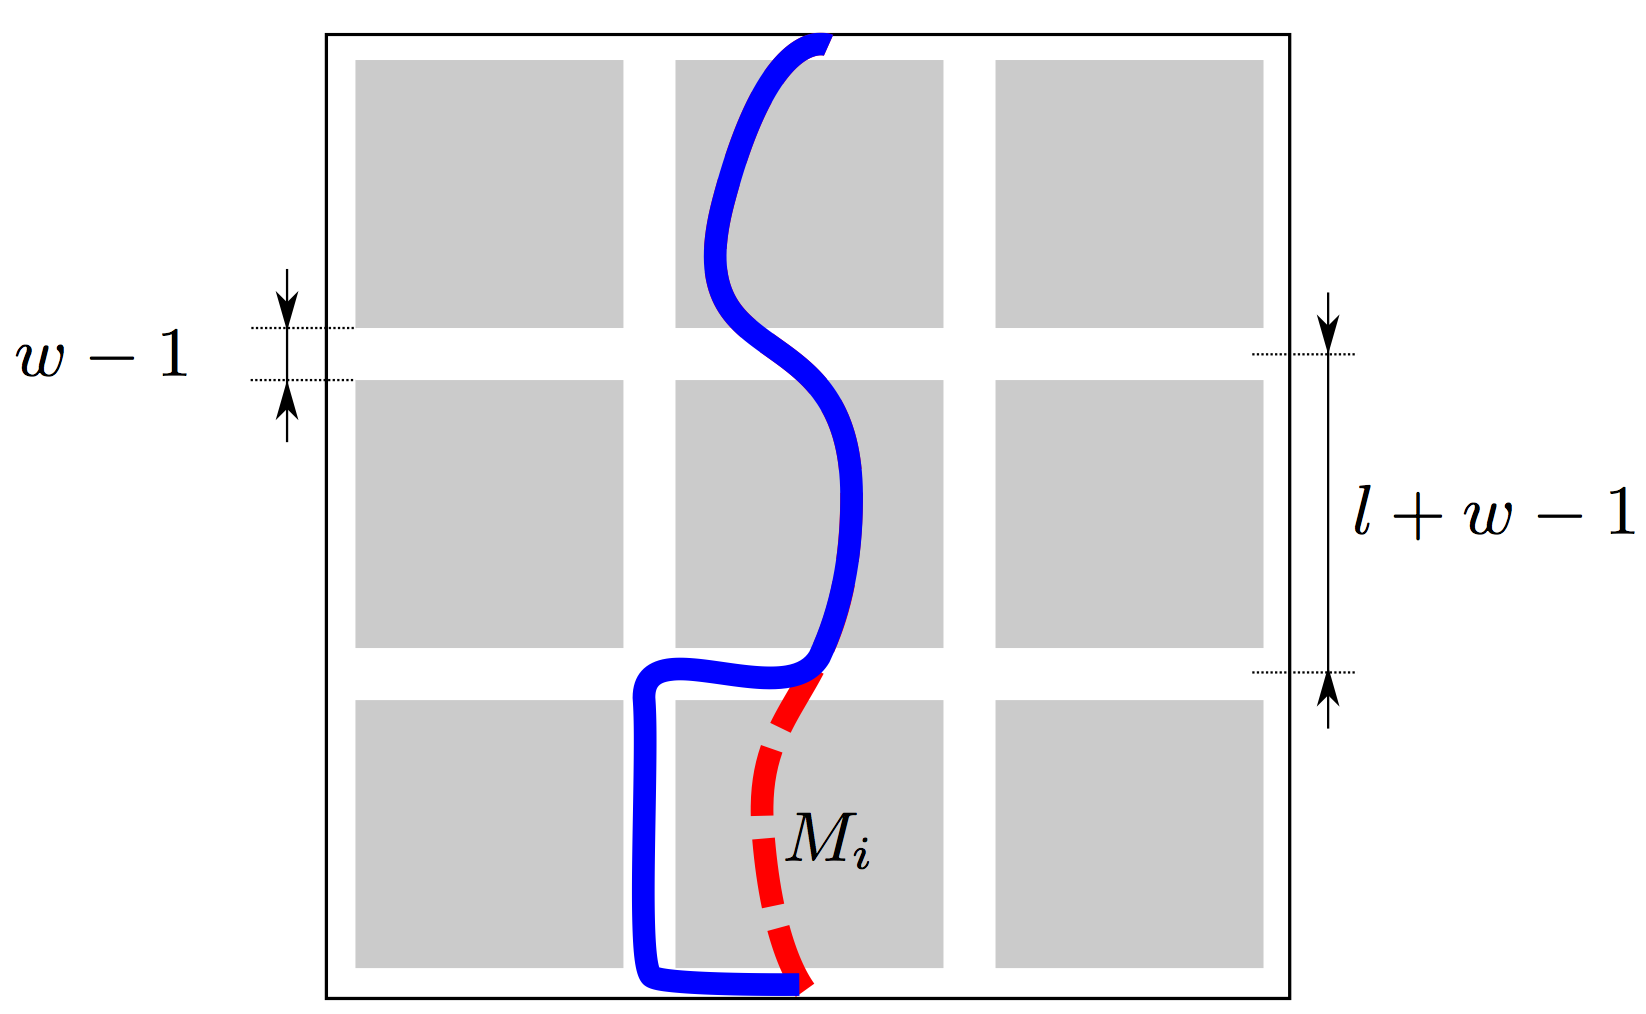
\includegraphics[width=0.42\textwidth]{lop_cleaning.png}
\caption{Lattice covering used in the proof of Theorem 1, shown in two dimensions. 
Each gray square is $l\times l$ and the white gap between squares has width $w-1$. 
The solid blue curve represents the support of a nontrivial logical operator; 
because the square $M_i$ is correctable, this square can be ``cleaned.'' 
We can find an equivalent logical operator supported on $M_i^c$, the complement of $M_i$. 
When all squares are cleaned, the logical operator is supported on the narrow strips between the squares.}
\label{fig:cleaning}
\end{figure}
%%%%%%%%%%%%%%%%%%%%%%%%%%%%%%%%%%%%%%%%%%%%%%%%%%%%%%%%%%%%%%%%

\begin{theorem}\emph{(Trade-off theorem for subsystem codes)}
For a local subsystem code in $D\ge 2$ dimensions with interaction range $w>1$ and distance $d\gg w$, 
defined on a hypercubic lattice with linear size $L$, 
every dressed logical operator is equivalent to an operator with weight $\tilde d$ satisfying
\begin{equation}\label{eq:tradeoff-bound}
  \tilde d {d}^{1/(D-1)} < c L^D,
\end{equation}
where $c$ is a constant depending on $w$ and $D$.
\label{thm:subsystem-tradeoff}
\end{theorem}

\begin{proof}
As shown in Fig.~\ref{fig:cleaning}, we fill the lattice with hypercubes, separated by distance $w-1$, 
such that each hypercube has linear size $l$ satisfying Eq.~\eqref{eq:hypercube-size}. 
(By ``distance'' we mean the number of sites in between --- e.g., we say that adjacent sites are ``distance zero'' apart.)
Thus no gauge generator acts nontrivially on more than one hypercube, 
and each hypercube is correctable by Lemma~\ref{lem:subsystem-hypercube}. 
Consider any nontrivial dressed logical operator $x$, 
and label the hypercubes $\{M_1, M_2, M_3, \dots\}$. 
By Lemma 3 there exists a gauge operator $y_i$ that ``cleans'' the logical operator in the hypercube $M_i$, 
i.e., such that $xy_i$ acts trivially in $M_i$. 
Furthermore, since no gauge generator acts nontrivially on more than one hypercube, 
we can choose $y_i$ so that it acts trivially in all other hypercubes. 
Taking the product of all the $y_i$'s we construct 
a gauge operator that cleans all hypercubes simultaneously; 
thus $\tilde x= x\prod_i y_i$ is equivalent to $x$ and supported on the complement of the union of hypercubes $M=\cup_i M_i$. 
Therefore, the weight $\tilde d$ of $\tilde x$ is upper bounded by $|M^c|$. 

The lattice is covered by hypercubes of linear size $l+(w-1)$, 
each centered about one of the $M_i$'s. 
There are $L^D/\left[l+(w-1)\right]^D$ such hypercubes in this union, 
each containing no more than $\left[l+(w-1)\right]^D - l^D \le (w-1)D\left[l+(w-1)\right]^{D-1}$ elements of $M^c$. 
Thus 
\[
\tilde d \le |M^c| 
\le (w-1)D\left[l+(w-1)\right]^{D-1}\frac{L^D}{\left[l+(w-1)\right]^D} 
= \frac{(w-1)D}{l+(w-1)}L^D.
\]
We optimize this upper bound on $\tilde d$ by choosing $l$ to be the largest integer 
such that a hypercube with linear size $l$ is known to be correctable,  
i.e., satisfying
\[
l < \left(\frac{d}{4(w-1)D}\right)^{1/(D-1)},
\]
thus obtaining Eq.~\eqref{eq:tradeoff-bound}.
Note that Eq.~\eqref{eq:tradeoff-bound} is trivial 
if $d$ is a constant independent of $L$, 
since the weight $\tilde d$ cannot be larger than $L^D$.
\end{proof}
